This document has the goal to report our analysis of the provided EEG data, collected during a MI experiment, and the simulation of a BCI loop. \\
Data has been recorded with 16-channel EEG amplifier (g.USBamp, g.Tec) @512Hz. Electrodes were placed accordingly to the 10-20 standard layout (Figure \ref{fig:electrodes_layout}). \\
Each subject participated in 3 recording days, performing  “offline” (calibration, no real feedback) and  “online” (with real feedback) runs. \\
The partecipants of the experiment were asked to perform two classes of MI tasks (both hands and both feet) while their EEG was collected, moreover some resting periods were also recorded.\\
The final purpose of a BCI such as this, is to train a system to recognize from EEG data, which MI task is performed.

\begin{figure}[h!]
	\begin{center}
		 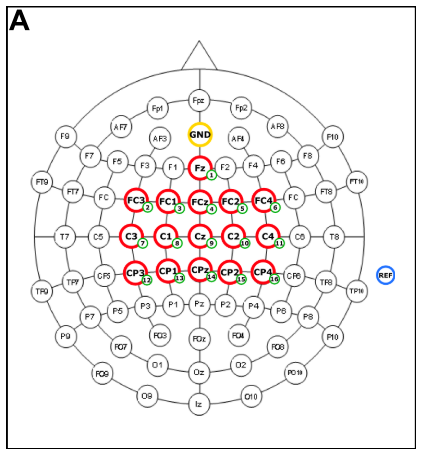
\includegraphics[width=0.4\linewidth]{img/electrodes_layout.PNG}
	\end{center}

	 \caption{Electrodes layout}
	 \label{fig:electrodes_layout}
\end{figure}